\documentclass[../report.tex]{subfiles}
\begin{document}

\subsection{Sample Data} \label{sec:sampledata}
	The first dataset is from an event in California on June 22nd 1987 at around 11:00 UTC recorded from 9 nearby stations. \cref{fig:calmap} shows a map of the stations extrapolated from the latitude and longitude in their metadata.  This dataset will be used to train the algorithm for detecting events as they have varying amounts of signal to noise ratio.
	
	\Cref{fig:calraw} shows the raw unprocessed traces from these stations (the X-axis shows seconds from 11:10:06 UTC).  As can be seen from these plots, there is a high variation of background noise and little obvious correlation between the shapes of the event as observed from different stations.
	
\begin{figure}[H]
	\centering
	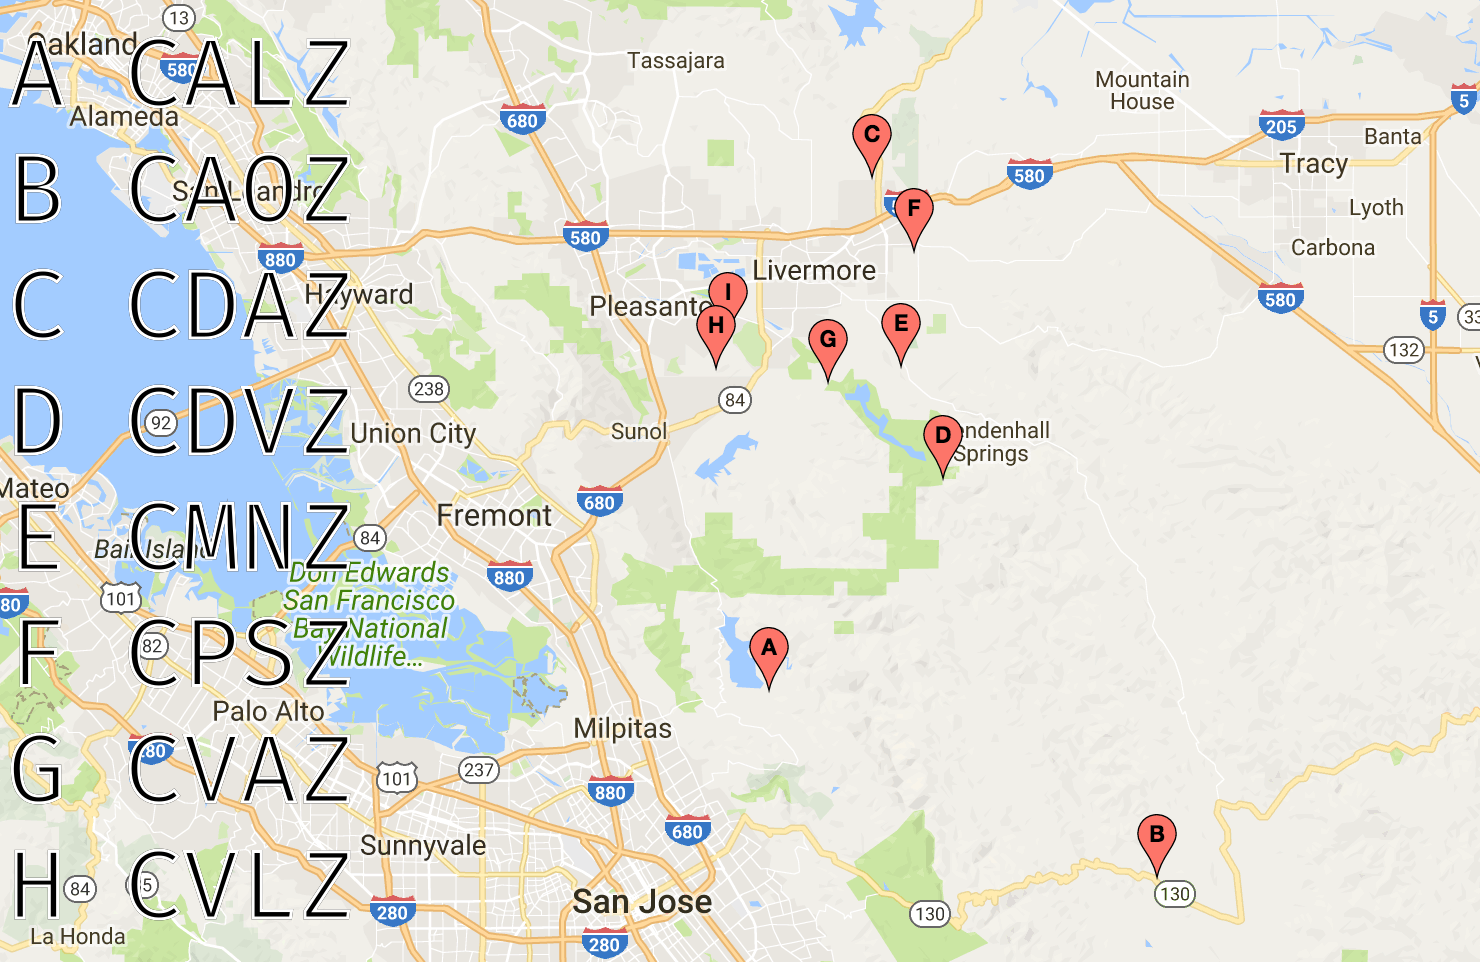
\includegraphics[width=0.7\linewidth]{img/cal-map-key}
	\caption{Map of Seismic Stations}
	\label{fig:calmap}
\end{figure}

\begin{figure}[H]
	\centering
	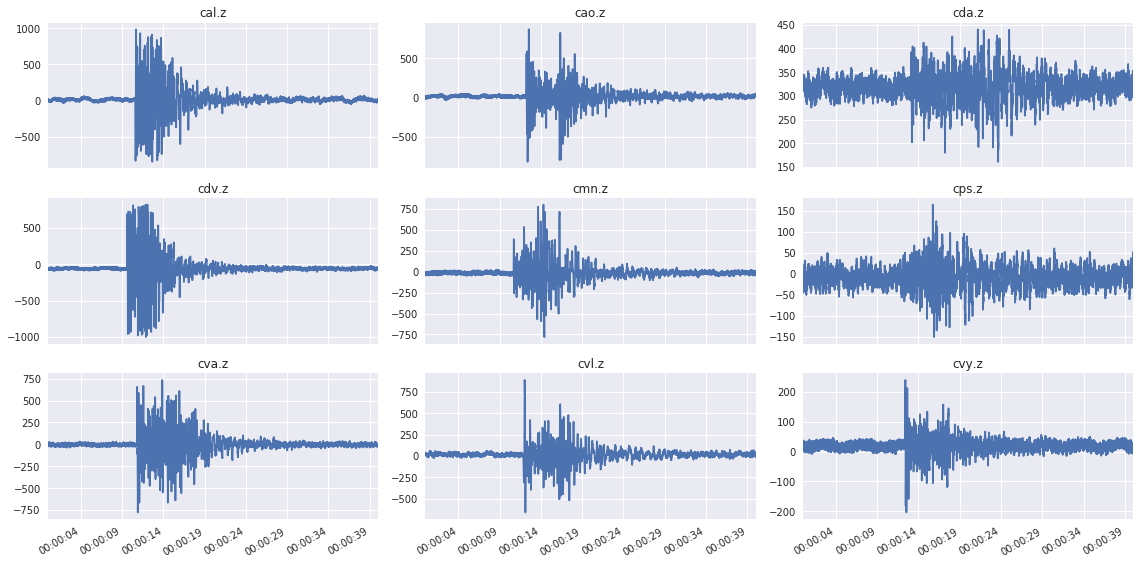
\includegraphics[width=1\linewidth]{img/cal_raw}
	\caption{Raw Observation Data}
	\label{fig:calraw}
\end{figure}

	The second dataset is from the Nabro volcano in Eritrea \citep{eritrea1}.  It consists of a years worth of observations from stations situated around the volcano.  Volcanoes sometimes produce similar waves when the event source is the same.  Within this dataset, known similarities have been provided between some events.  These events (totalling 138) will be used to evaluate the similarity measures.

\subsection{Frequency filtering (Butterworth Bandpass)}
	As seen in \cref{sec:sampledata} and \cref{fig:calraw}, raw seismic traces contain a lot of background noise.  This consists of both high frequency and low frequency interference which can be cause by many unrelated events such as wind, temperature variations and human events such as traffic and construction work.  A commonly used technique \citep{man-seis-obs} is to perform a Butterworth Filter \citep{bandpass} on the data, eliminating frequencies that are outside of a given range.  The most significant frequencies from a seismic event tend to be between 5 and 10Hz so these values are used going forwards to clean the data.  The bandpass filter is provided by the Obspy library and implemented as a method in the \verb|ObservationDAO| class.
	
	The effects of applying the bandpass filter can be seen in \cref{fig:calbandpass}.  This results a much cleaner event profile however there is unfortunately still little obvious visual correlation beyond timing between the observations.

\begin{figure}[H]
	\centering
	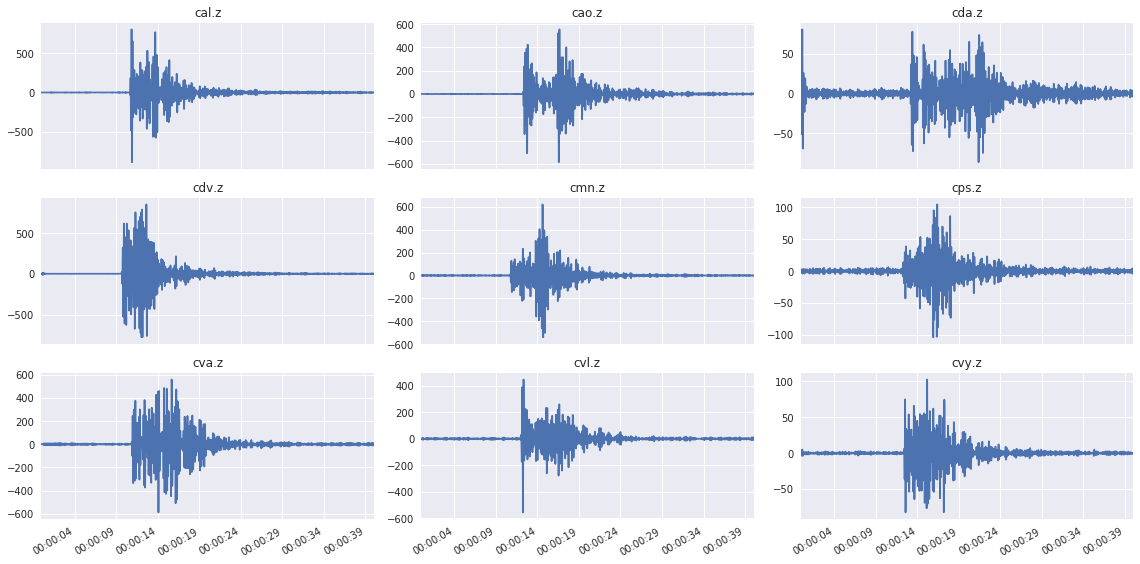
\includegraphics[width=1\linewidth]{img/cal_bandpass}
	\caption{Frequency Filtered Observation Data (5-10Hz)}
	\label{fig:calbandpass}
\end{figure}

\end{document}